\documentclass[
%11pt, % The default document font size, options: 10pt, 11pt, 12pt
%oneside, % Two side (alternating margins) for binding by default, uncomment to switch to one side
english, % ngerman for German
%singlespacing, % Single line spacing, alternatives: onehalfspacing or doublespacing
%draft, % Uncomment to enable draft mode (no pictures, no links, overfull hboxes indicated)
%nolistspacing, % If the document is onehalfspacing or doublespacing, uncomment this to set spacing in lists to single
%liststotoc, % Uncomment to add the list of figures/tables/etc to the table of contents
%toctotoc, % Uncomment to add the main table of contents to the table of contents
%parskip, % Uncomment to add space between paragraphs
%nohyperref, % Uncomment to not load the hyperref package
headsepline, % Uncomment to get a line under the header
%chapterinoneline, % Uncomment to place the chapter title next to the number on one line
%consistentlayout, % Uncomment to change the layout of the declaration, abstract and acknowledgements pages to match the default layout
]{scrartcl} % The class file specifying the document structure

\usepackage[utf8]{inputenc} % Required for inputting international characters
%\usepackage[T1]{fontenc} % Output font encoding for international characters
\usepackage{hyperref, lipsum} % libs for clickable links and generating dummy text
\usepackage[toc,page]{appendix} % appendix commands \appendix. not used rn 
\usepackage{graphicx, graphbox, subcaption} 
\usepackage{biblatex}
\usepackage{siunitx, booktabs}
\graphicspath{ {./images/} }
\usepackage{multicol}
\usepackage{multirow}
\usepackage{array}
    \newcolumntype{P}[1]{>{\centering\arraybackslash}p{#1}}
    \newcolumntype{M}[1]{>{\centering\arraybackslash}m{#1}}
    \newcolumntype{L}[1]{>{\raggedright\arraybackslash}m{#1}} %% left aligned
    \newcolumntype{C}[1]{>{\centering\arraybackslash}m{#1}}   %% centered
    \newcolumntype{R}[1]{>{\raggedleft\arraybackslash}m{#1}}  %% right aligned
\usepackage{stackengine}
    \newcommand\xrowht[2][0]{\addstackgap[0.5\dimexpr#2\relax]{\vphantom{#1}}}

\usepackage{listings}
\usepackage{color}
    \lstloadlanguages{C,[Sharp]C,C++,csh,Java}
    
    \definecolor{bluekeywords}{rgb}{0.13,0.13,1}
    \definecolor{greencomments}{rgb}{0,0.5,0}
    \definecolor{redstrings}{rgb}{0.9,0,0}

    \lstset{
    language=[Sharp]C,
    showspaces=false,
    showtabs=false,
    breaklines=true,
    showstringspaces=false,
    breakatwhitespace=true,
    escapeinside={(*@}{@*)},
    commentstyle=\color{greencomments},
    keywordstyle=\color{bluekeywords}\bfseries,
    stringstyle=\color{redstrings},
    basicstyle=\ttfamily
    }

\usepackage{caption}
    \DeclareCaptionFont{white}{\color{white}}
    \DeclareCaptionFormat{listing}{\colorbox{blue}{\parbox{\textwidth}{\hspace{15pt}#1#2#3}}}
    \captionsetup[lstlisting]{format=listing,labelfont=white,textfont=white, singlelinecheck=false, margin=0pt, font={bf,footnotesize}}

\usepackage{amsmath}
\usepackage{bm} % to display math in bold.
\usepackage{todonotes}

\begin{document}
\begin{titlepage}
\title{Exploration and Presentation Assignment 2}
\author{Simon Bojesen - cph-sb339@cphbusiness.dk}
\subtitle{Task 2}
\maketitle
\begin{center}
    \large
        Copenhagen Business Academy\\
        Supervisor: Dr. Super Visor\\
        Examiner: Mr. Exam Miner
\end{center}

\thispagestyle{empty}

\end{titlepage}
\clearpage

\pagenumbering{arabic}
\Large
    \textbf{Abstract}
    \begin{abstract}
        \label{sec:abstract}
        This is where an abstract will be in 4 sentences! What is the problem? Why is the problem interesting? What is the solution? 
        What are the implications of the solution?
    \end{abstract}
\normalsize  
\clearpage

\section{Introduction}
\label{sec:introduction} % Don't use bold this way in the actual report - only for template purpose.
    \textbf{Most of this document's review material is to be found in section \ref{sec:Assignment Tasks}.
    \todo{Tell reviewer what to look at so they don't waste time on all the sections irrelevant to the assignment.}\\    
    Otherwise see the unnumbered section right after section 2 and the bibliography.}\\ 
    \textbf{Motivation} — Why this topic is important nowadays.\\
    \textbf{Project objectives} — what is the expected result.\\
    \textbf{Project tasks} — what is to be done for achievement of the objectives -steps  in  the  work, 
        such  as  getting  acquainted  with  the  state-of-the-art and  trends  in  the  area,  
        selecting  a  development  methodology,  creatinga  design,  selecting  development  tools  and  environments,  
        programming,testing, implementation and evaluation, as appropriate.\\
    \textbf{Scope of the project} — what is not an objective or a task.\\
    \textbf{Brief description of the other chapters that follow} — one paragraph per each.
\clearpage

\tableofcontents % Prints the main table of contents

\listoffigures % Prints the list of figures

\listoftables % Prints the list of tables

\section{Assignment Tasks} 
\label{sec:Assignment Tasks}
    A demonstration of some international symbols working: æ ø å Æ Ø Å µ ü ö Ü Ö.

    See the figure \ref{fig:HelixNebula} on page \pageref{fig:HelixNebula} to see a picture of the Helix Nebula.
 \subsection{Assignment Subsection}
 \label{sec:Assignment Subsection}
    \subsubsection{Assignment Subsubsection}
    \label{sec:Assignment Subsubsection}
        \begin{paragraph}           
            assignment paragraph beginning.
            \begin{subparagraph}
                assignment subparagraph.\\
            \end{subparagraph}
            assignment paragraph ending.
        \end{paragraph}

    \subsection{Assignment Lists}
        List with bullet points:
        \begin{itemize}
            \item Item A.
            \item Item B.
            \item Item C.
        \end{itemize}
        List with alternate symbols:
        \begin{itemize}
            \item[--] Item A.
            \item[--] Item B.
            \item[--] Item C.
        \end{itemize}
        Numbered List:
        \begin{enumerate}
            \item Item A.
            \item Item B.
            \item Item C.
        \end{enumerate}

    \subsection{Assignment Tables}
    \begin{table}[ht]
        \caption{Multi-column and multi-row table}
        \caption*{\footnotesize Smaller note of table that describes what the table is all about.}
        \begin{center}
            \begin{tabular}{lcr} % left center and right alignment. Example of bigger table below with predefined column types.
                \hline
                \multicolumn{2}{c}{\multirow{2}{*}{Multi-col-row}}&X\\ % Both multicolumn and multirow used.
                \multicolumn{2}{c}{}&X\\
                \hline
                X&X \vline &  \multirow{2}{*}{X}\\ % Single column multirow
                X&X \vline \\
                \hline
            \end{tabular}
        \end{center}
        \label{tab:multicol}
    \end{table}
    \begin{table}
        \renewcommand\arraystretch{1.3}
        \begin{center}
        \begin{tabular}{ | L{\dimexpr 0.3\linewidth-2\tabcolsep} | C{\dimexpr 0.3\linewidth-2\tabcolsep} | R{\dimexpr 0.3\linewidth-2\tabcolsep} | }  
        \hline
            LEFT TEXT LEFT 
            TEXT LEFT TEXT  
            LEFT TEXT LEFT 
            TEXT LEFT TEXT 
            &
            MORE CENTER TEXT
            &
            RIGHT TEXT \\
        \hline
            LEFT TEXT
            &
            CENTER TEXT CENTER  
            TEXT CENTER TEXT 
            CENTER TEXT CENTER  
            TEXT CENTER TEXT 
            &
            I BELIEVE IN RIGHT TEXT
             \\
        \hline
            I BELIEVE IN LEFT TEXT
            &
            CENTER TEXT
            &
            RIGHT TEXT RIGHT  
            TEXT RIGHT TEXT  
            RIGHT TEXT RIGHT  
            TEXT RIGHT TEXT \\
        \hline
        \end{tabular}
        \end{center}
    \end{table}
    Here is a reference to the multi-column and multi-row table \ref{tab:multicol}.
    
    \subsection{Assignment Code Listings}
        \begin{lstlisting}[language={[Sharp]C}, caption={C\# example}, label={Script}]
            //Prints Hello World.
            class Program
            {
              public static void Main()
              {
                System.Console.WriteLine("Hello World!");
              }
            }
        \end{lstlisting}

    \subsection{Assignment Math equations}
        As an example of inline equations, here is once again the equation for the maximum page count for the report: 
        $\bm{maxPageCount = 40 + 20 \cdot numberOfStudents}$. 
        And text on the other side of the equation. If you should want it on another line, you can use the amsmath package like so:\\
        Example for \texttt{gather}:
        \begin{gather}
            \vec{F} = \binom{5\cdot \cos( \frac{\pi}{5})}{5\cdot \sin( \frac{\pi}{5})}=\binom{4.04}{2.93}\\
            \sqrt{F_x^2 + F_y^2} = \sqrt{4.04508497187^2 + 2.93892626146^2} = 4.99999999999
        \end{gather}
        Example for \texttt{align}:
        \begin{align}
            \vec{F} = \binom{5\cdot \cos( \frac{\pi}{5})}{5\cdot \sin( \frac{\pi}{5})}=\binom{4.04}{2.93}\\
            \sqrt{F_x^2 + F_y^2} = \sqrt{4.04508497187^2 + 2.93892626146^2} = 4.99999999999
        \end{align}
        Let’s say we want to print out the sum of $n^2$ for n between 1 and 10. To do this we would do the following:\\
        \begin{align}
            \sum_{n=1}^{10} n^{2}
            \label{sumExample}
        \end{align}
        And a product sequence:
        \begin{align}
            \prod_{x=1}^{n}x^{2}
            \label{prodExample}
        \end{align}



\section*{Unnumbered Assignment Section}
\label{sec:Unnumbered Assignment Section}
    This section isn't in the table of contents.


\begin{figure}
    \caption{A picture of the Helix Nebula.} % Caption on top of both of the images.
    \centering % Centering requirement met
    \begin{subfigure}[b]{0.3\textwidth}
        \includegraphics[width=\textwidth]{HelixNebula.jpg}
        \caption{A picture of the Helix Nebula.} % caption under a.
        \label{fig:HelixNebula}
    \end{subfigure}
    \begin{subfigure}[b]{0.3\textwidth}
        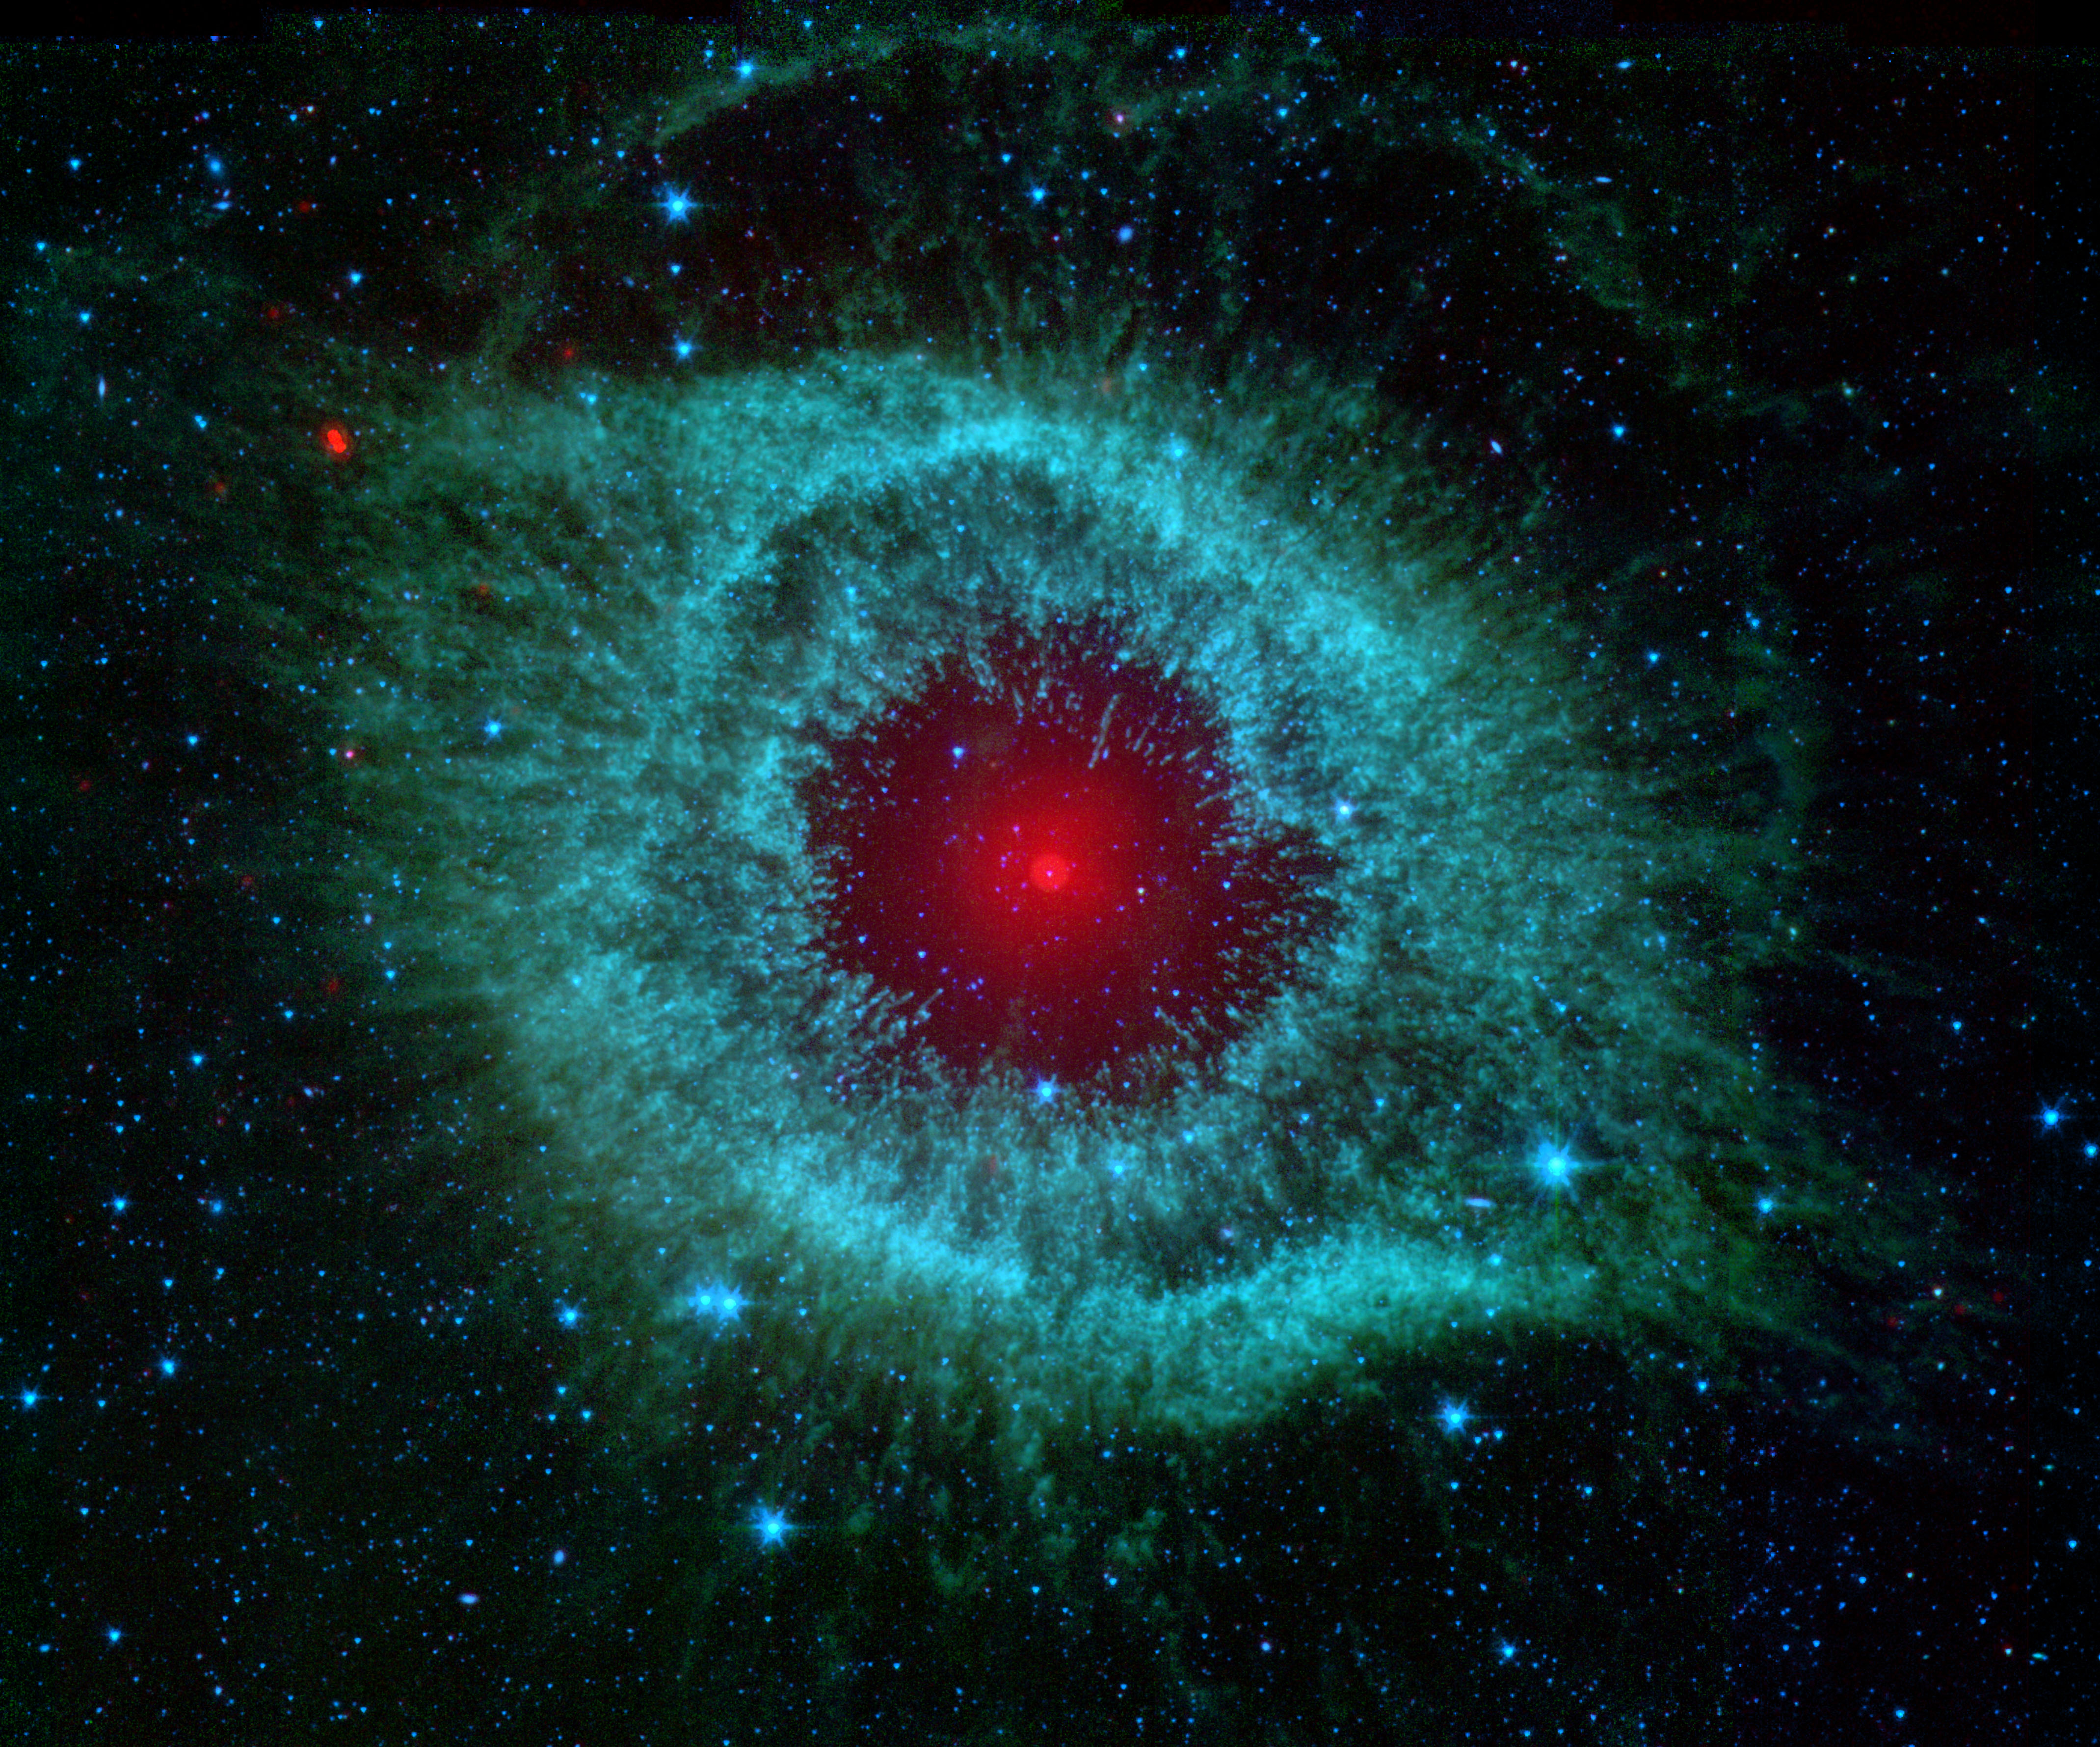
\includegraphics[width=\textwidth]{InfraredHelixNebula.jpg}
        \caption{A picture of the Helix Nebula in infrared.} % caption under b.
        \label{fig:InfraredHelixNebula}
    \end{subfigure}
  \end{figure}

\section{State of the art and trends}
\label{sec:State of the art and trends}
    Survey of current technologies and similar solu-tions in this area – to show that you are well informed and step on the availableachievements: 
    For  example,  you  can  present  some  relevant  knowledge  gath-ered from both previously studied modules and external sources, organized in astructured form.  
    Here you can also describe and compare alternative develop-ment methodologies, technologies, environments, frameworks, or programming2
    languages  that  could  have  been  used,  and  to  explain  and  argue  your  choice.Inside the  text,  a citation or a reference  to the used  sources (books,  articles,web pages) is required.  The sources can be listed either underscore,  or in an Appendix.

\section{Requirements specification and solution design}
\label{sec:Requirements specification and solution design}
    Formulation of projectfoundation – a solid ground of your solution:This part reflects the design pro-cess, or the methodology you have followed. 
    Analysis – who are the users, usecases  and  scenarios,  intended  user  experiences.  The  analysis  lead  to  specifi-cations – formal functional and 
    non-functional requirement to the application.Specifications  lead  to  requirements:  you  consider  how  to  design  the  solution– system architecture, 
    data models, visual interface, control, operability, algo-rithms,  integration  and  other  components,  as  appropriate. 
    Use  graphics  forvisual presentation of your concepts as much as possible.

\section{Solution development and implementation}
\label{sec:Solution development and implementation}
    Presentation of the applica-tion, test procedures, deployment and maintenance environments:This part presents the product in technical terms. 
    Implementation and test environment — test strategies, test plan, test suites, demo and screen captures, usability evaluation, etc. 
    Units of code, packages, deployment, supported interfaces, al-gorithms,  input  and  output,  supported  file  formats,  frameworks,  servers  andclients, etc.

\section{Conclusions}
\label{sec:Conclusions}
    Brief summary:What  has  been  done  and  the  benefits  of  it. Recommendation for future extensions and upgrades. Reflection on the workand the product.


\section{Rules and recommendations to Remember}
\label{sec:Rules and recommendations to Remember}
    In the \href{https://datsoftlyngby.github.io/soft2020fall/resources/bbe51cf2-bachelorProject.pdf}{recommendations and requirements pdf} the following rules, recommendations and explanations are laid out:
    \begin{itemize}
        \item Strive to \textbf{include elements from courses passed}.
        \item Group size is \textbf{maximum 4 students}. Larger groups carry larger expectations.
        \item The 15 ECTS points the project covers should amount to \textbf{412.5 hours} of project work.
    \end{itemize}

    \subsection{Report}
    \label{sec:report}
        As before, the Report requirements are found in the \href{https://datsoftlyngby.github.io/soft2020fall/resources/bbe51cf2-bachelorProject.pdf}{recommendations and requirements pdf}.
        \begin{enumerate}
            \item The maximum page count for the report is:\\$maxPageCount = 40 + 20 \cdot numberOfStudents$.\\
                Meaning that a single student can write up to 60 pages and two students can write 80, etc.
            \item The report can be written in either \textbf{Danish or English}.
            \item The report \textbf{must} contain a thorough description of the work that has been done during the bachelor project, 
                as well as an evaluation and reflectionon the work.
        \end{enumerate}

    \subsection{Final  works}
    \label{sec:Final  works}
        Project and documentation completed. Visual (power point) presentation and a demo prepared. 
        It is recommended to discuss the draft of the report with the supervisor before the final!

    \subsection{Other Handy Things}
    This section is just for handy things to remember for later that are not required by the assignment.
    \label{sec:Other Handy Things}
        \begin{table}
            \caption{The effects of treatments X and Y on the four groups studied.}
            \label{tab:treatments}
            \centering
            \begin{tabular}{l l l}
                \toprule
                {Groups} & {Treatment X} & {Treatment Y}\\
                \midrule
                1 & 0.2 & 0.8\\
                2 & 0.17 & 0.7\\
                3 & 0.24 & 0.75\\
                4 & 0.68 & 0.3\\
                \bottomrule\\
            \end{tabular}
        \end{table}
        See Table \ref{tab:treatments}.

\begin{appendices}
    \section{Appendix A}
    \label{sec:Appendix A}
    %\input{appendixA} % filename in curly brackets - Requires a .tex file with the name.
    \section{Appendix B}
    \label{sec:Appendix B}
    %\input{appendixB} % filename in curly brackets - Requires a .tex file with the name.
    \clearpage
\end{appendices}

\begin{thebibliography}{9}
\label{thebibliography}
    \bibitem{FirstBook} 
    Author A, Author B and Author C. 
    \textit{The First Book Name}. 
    Publisher 1, Reading, City Name, Year.
    
    \bibitem{How to get a paper accepted at oopsla} 
    Kent Beck. 
    \textit{How to get a paper accepted at oopsla, 1993}
    
    \bibitem{Studieordning} 
    Copenhagen Business Academy.\\
    \textit{Studieordning  for  professionsbacheloruddannelsen  i  soft-wareudvikling}. (Danish) 
    [\textit{Curriculum forthe Bachelor’s Degree Programme in Software Development, aug 2017}].
    \\\url{https://datsoftlyngby.github.io/soft2020fall/resources/bbe51cf2-bachelorProject.pdf}
\end{thebibliography}

\end{document}